
\documentclass[dvipdfmx]{standalone}
\usepackage[T1]{fontenc}
\usepackage{lmodern}
% \usepackage{newtxtext, newtxmath}

\usepackage{tikz}

\begin{document}
  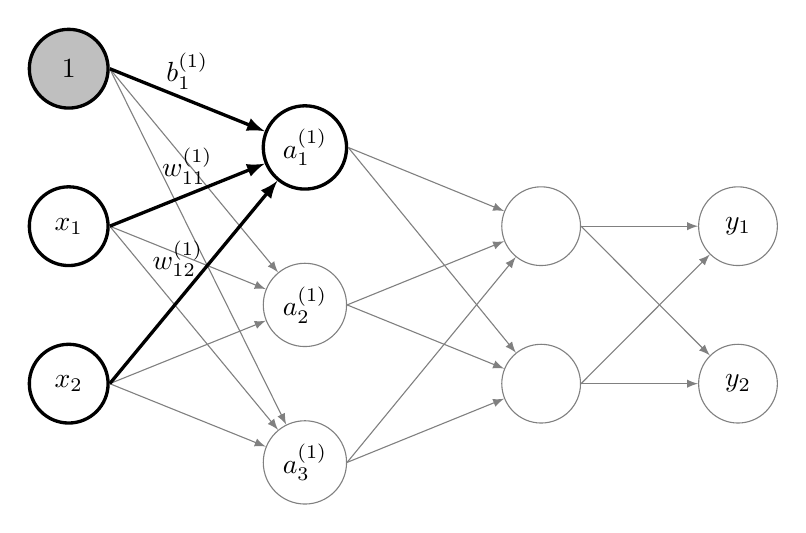
\begin{tikzpicture}[color=gray]
    \tikzset{
      neuralnode/.style={color=black, circle, draw=gray, minimum size=1cm, align=center},
      network/.style={->, > = latex},
      focus/.style={draw=black, color=black, very thick}
    }
    \draw (0,6) node (b1) [neuralnode, focus, fill=gray!50] {1}; % bias
    \draw (0,4) node (x1) [neuralnode, focus] {$x_1$};
    \draw (0,2) node (x2) [neuralnode, focus] {$x_2$};
    \draw (3,5) node (a1) [neuralnode, focus] {$a_1^{(1)}$};
    \draw (3,3) node (a2) [neuralnode] {$a_2^{(1)}$};
    \draw (3,1) node (a3) [neuralnode] {$a_3^{(1)}$};
    \draw (6,4) node (c1) [neuralnode] {};
    \draw (6,2) node (c2) [neuralnode] {};
    \draw (8.5,4) node (y1) [neuralnode] {$y_1$};
    \draw (8.5,2) node (y2) [neuralnode] {$y_2$};

    \foreach \from in {b1, x1, x2}
      \foreach \to in {a2, a3}
        \draw[network] (\from.east) -- (\to);
    \begin{scope}[label distance=0.2cm]
      \draw[network, focus] (b1.east) -- node [above] {$b_1^{(1)}$} (a1);
      \draw[network, focus] (x1.east) -- node [above] {$w_{11}^{(1)}$} (a1);
      \draw[network, focus] (x2.east) -- node [xshift=-2mm, yshift=3mm] {$w_{12}^{(1)}$} (a1);
    \end{scope}
    \foreach \from in {a1, a2, a3}
      \foreach \to in {c1, c2}
        \draw[network] (\from.east) -- (\to);
    \foreach \from in {c1, c2}
      \foreach \to in {y1, y2}
        \draw[network] (\from.east) -- (\to);

  \end{tikzpicture}
\end{document}
